\chapter{Analýza požiadaviek systému}

Hlavnou úlohou navrhovaného systému je umožniť užívateľovi pohodlne pracovať na odhaľovaní parsovacích vzorov použitím Recursive User-Reviewed Clustering cyklu a algoritmu Extended Nagappan-Vouk. Užívateľské rozhranie musí byť prívetivé a informovať používateľa o prípadných chybách počas analýzy logovacích správ.

\section{Užívateľské akcie -- prípady užitia}

Systém automaticky predpokladá, že užívateľ má pri prístupe v pláne začať analyzovať logovacie správy, a preto je presmerovaný na záložku Miner do stavu začatia novej analýzy. 
\par V tomto stave môže užívateľ zadať zdroj dát, z ktorého budú pochádzať dáta analyzované v ďalšom kroku, alebo tento krok preskočiť. Následne môže ako zdroj vstupných dát vybrať logovací súbor alebo použiť nespracované logovacie správy, ktoré sú v systéme uložené. Dostupné sú aj nastavenia algoritmu, ktoré sú špecifické pre nasledovný beh analýzy. \par Užívateľovi sú potom prezentované nájdené parsovacie vzory, ktoré môže potvrdiť a rozhodnúť, ako s nimi ďalej pracovať. Rovnako si môže nájdené vzory prehliadnuť, zobraziť správy, ktoré k nemu patria, prípadne daný vzor odstrániť. Nájdené vzory sa dajú filtrovať podľa zdroja správ a vyexportovať.

\begin{figure}[htbp]
 \centering 
 \begin{minipage}{0.95\linewidth}
 	\centering
 	\missingfigure[figheight=12cm]{Text}
 	%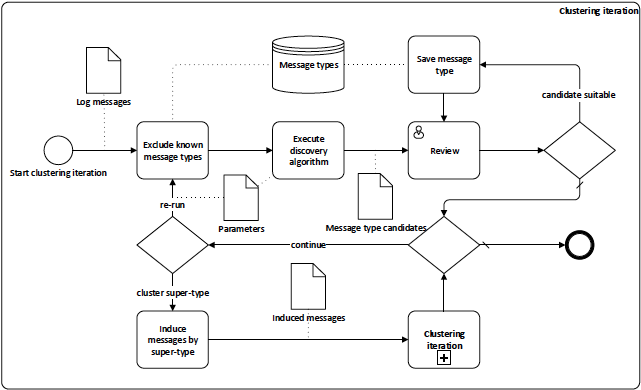
\includegraphics[width=\textwidth]{images/RURC.png} 	
 \end{minipage}
  \caption{Use case }
  \label{fig:use-cases}
\end{figure}

\section{Komponenty systému}
Po preskúmaní požiadaviek sme dospeli k záveru, že systém vieme ďalej rozdeliť do týchto kategógií:

\begin{enumerate}
  \item Task queue
  \item Webový backend
  \item Úložisko dát
  \item Užívateľské rozhranie
\end{enumerate}

\subsection{Užívateľské rozhranie}
Užívateľské rozhranie musí byť intuitívne a poskytovať dobrú podporu pre asynchrónne operácie, ktoré bude spúšťať. RURC proces definovaný v \ref{sec:rurc} môže byť v budúcnosti ešte rozšírený, a preto je zároveň dôležité, aby sa užívateľské rozhranie dalo jednoducho rozšíriť a zdrojový kód udržovať.

\subsection{Webové API}
Backend bude prijímať a spracovávať požiadavky od klienta. Musí vedieť persistovať dáta, spúštať dlhotrvajúce úlohy na task queue a poskytovať klientovi možnosť zistiť status bežiacej úlohy. Mala by byť použitá dobre známa technológia, ktorá sa dobre integruje a umožňuje rýchly vývoj.

\subsection{Task queue}
Task queue je zodpovedná za beh dlhotrvajúcich operácií. Dôležitými vlastnosťami sú preto stabilita, výkonnosť a schopnosť zotaviť sa z chyby. Je podstatné, aby po výskyte chyby v jednom behu úlohy nebola ovplyvnená schopnosť prijímať ďalšie. Je tu zároveň požiadavka na možnosť dopytovať sa na stav bežiacej úlohy.

\subsection{Úložisko dát}
Dáta, s ktorými sa v aplikácii pracuje, sú z relačného pohľadu jednoducho štruktúrované. Veľkú časť dát tvoria medzivýsledky, ktoré potrebujeme vedieť rýchlo spracovať a uložiť, keďže po krátkom čase budú zo systému zmazané. V tomto pípade sa naskytá otázka, či sa má použiť tradičná relačná databáza alebo niektorá z NoSQL databáz. 

\section{Technologické riešenie}

Extended Nagappan-Vouk algoritmus aj RURC cyklus sú dostupné pod slobodnou softvérovou licenciou. Rovnako by pod slobodnou licenciou mali byť aj všetky technológie a nástroje použité na implementáciu a beh systému, aby bol býsledný systém ľahko nasaditeľný a dostupný.


\subsection{Programovací jazyk}
Ako programovací jazyk systému sme po úvahe zvolili Python. 
\par Python predstavuje rozšírený a populárny dynamicky typovaný jazyk, ktorý patrí medzi základnú sadu programov nainštalovaných na väčšine linuxových distribúcií. Medzi jeho prednosti patrí široká škála voľne dostupných knižníc a jednoduchá správa závislostí, napr. použitím balíčkovacieho správcu pip. Navyše je používaný v už existujúcich systémoch ÚVT, rovnako ako aj v referenčnej implementácii spomínaných algoritmov, čo predstavuje ďalšie dôvody pre jeho výber. 

\subsection{Task queue}
Užívateľ si v klientskej časti navolí parametre a klient spustí pomocou http volania API algoritmus hľadania parsovacích vzorov.
\par Dĺžka behu spustenej analýzy je silne závislá od počtu vstupných logovacích správ, čo ale skoro vždy predstavuje časovo náročnú operáciu. Keďže klientska aplikácia by na výsledky nemala čakať až do dokončenia analýzy, je potrebné zvoliť riešenie, ktoré túto analýzu spustí na pozadí a ponúkne nám možnosť získať výsledky neskôr.
\par Task queue je systém pre paralelné vykonávanie úloh neblokujúcim spôsobom a pre svoje fungovanie využíva tieto komponenty :

\begin{enumerate}
  \item Broker -- prostredník, ktorý drží zadané úlohy.
  \item Producent -- funkcia, ktorá vytvára úlohy a posiela ich na brokera na neskoršie spracovanie.
  \item Konzument, ktorý vezme úlohy z brokera a vykoná ich. Neformálne si konzumenta môžeme predstaviť ako jedno vlákno, ktoré čaka na spustenie úlohy.
\end{enumerate}

Pre implementáciu task queue sme vybrali Celery. 
\par Celery predstavuje dobre zdokumentované a v súčasnej dobe asi najpoužívanejšie riešenie, ktoré síce je oproti ostatným variantom komplikovanejšie, ale vyniká vo výkone a stabilite. 
\par Ako broker sa odporúča využiť RabbitMQ alebo Redis. Vybrali sme Redis, a to predovšetkým pre jeho možné využitie ako úložisko dát, ako je spomenúté v \ref{sec:store}.

\subsection{Webový backend}
Pri výbere technológie pre webový backend sme brali do úvahy podporu technológie pre prácu s Celery a následne aj formu, ktorou bude vytvorené užívateľské rozhranie. Rozhodovali sme sa medzi dvoma najzámejšími frameworkami pre Python, konkrétne medzi frameworkami Django a Flask.
\par Django je viac robustné a poskytuje programátorovi väčšiu podporu, ale aj väčšie obmedzenia. Flask je zase jednoduchý framework, ktorý necháva programátorovi väčšiu voľnosť.
\par Oba frameworky podporujú pohodlnú prácu s Celery, no vďaka dobrej osobnej skúsenosti sme nakoniec zvolili Django.

\subsection{Úložisko dát}
\label{sec:store}
Pre ukladanie dát sme sa rozhodli použiť kombináciu relačnej databázy PostgreSQL a in-memory databázu Redis. 
\par PostgreSQL je open source databáza, ktorá plne implementuje štandard ANSI SQL a spĺňa vysoké nároky súčasne na konzistenciu dát a výkon. Hoci je PostreSQL rozsiahly systém s množstvom nastavení pre ladenie výkonu, je veľmi ľahko nainštalovateľný a už v základnom nastavení poskytuje dobrú výkonnosť. Navyše, aj framework Django odporúča pri výbere databázy použiť práve PostgreSQL, čo považujeme za výhodu.
\par Redis už v infraštuktúre máme použitý ako broker pre Celery, no okrem toho predstavuje veľmi rýchle in-memory úložisko typu kľúč-hodnota. Poskytuje sadu datových typov, ktorá je postačujúca na uloženie medzivýsledkov a asynchrónne ukladanie dát na disk.
\par Vo výsledku teda použijeme Redis pre uloženie všetkých neštrukturovaných dát a medzivýsledkov a PostgreSQL na prácu so štukturovanými dátami. To nám umožňuje dosiahnuť vysoký výkon v prípade potreby.

\subsection{Užívateľské rozhranie}
Pretože Django poskytuje pomerne dobré templatovacie možnosti, rozhodli sme sa túto možnosť využiť ako základ rozhrania.
\par Na dosiahnutie interaktivity a asynchrónnosti je však nutné použiť JavaScript. Vybrali sme preto knižnicu jQuery, ktorá sa ľahko integruje a pracuje dobre v kombinácií s Djangom. Týmito technológiami bol vytvorený funkčný prototyp, ktorý odhalil určité nedostatky. Pre naimplementovanie zobrazovania výsledných parsovacích vzorov bolo nutné použiť stromovú štruktúru, v ktorej sme potrebovali pridávať a odoberať uzly na užívateľom zvolenenom mieste v strome. Práca s týmto stromom bola s knižnicou jQuery síce možná, ale obslužný kód bol zbytočne komplikovaný a zle udržovateľný. Preto sme sa rozhodli túto kombináciu nahradiť čisto JavaScriptovým riešením. Bola zvolená knižnica Angular 2, ktorá je zameraná na vývoj interaktívnych aplikácií, umožňuje krátky vývojový proces a má veľkú sadu vývojárskych nástrojov.
\par Na štýlovanie užívateľského rozhrania sme použili Bootstrap. Jedná sa o momentálne najpoužívanejšie riešenie pre tvorbu moderných a responzívnych webov. To umožnilo, že výsledné rozhranie je z veľkej miery responzívne, aj keď nepredpokladáme jeho časté využitie na mobilných zariadeniach.

\begin{figure}[htbp]
 \centering 
 \begin{minipage}{0.95\linewidth}
 	\centering
 	\missingfigure[figheight=10cm]{diagram komponent}
 	%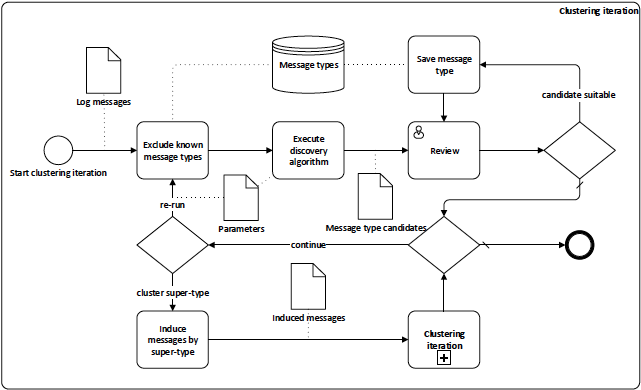
\includegraphics[width=\textwidth]{images/RURC.png} 	
 \end{minipage}
  \caption{Komponenty aplikácie }
  \label{fig:components}
\end{figure}

\section{Implementácia systému}
Štruktúru zdrojových kódov sme sa rozhodli rozdeliť na tri časti.
\par Serverová časť obsahuje zdrojové kódy v Pythone pre backend a producentov úloh pre Celery. Klientska časť zapuzdruje užívateľské rozhranie v Angular 2 a nástroje potrebné na vývoj a preklad zdrojových kódov. V inštalačnej časti sú skripty, ktoré plne automatizujú nasadenie aplikácie na linuxový server.